\chapter{System Design and Implementation}

This chapter describes of the system. It starts by providing overview of the system, followed by requirement elicitation to build prototype. Furthermore, it also provide deeper understanding of architectural paradigm by discussing each module and their interconnection.

\section{Overview}

Pervious chapter limits our discussion about the design decision and describe the essential component of the system.  Since the concept is quite abstract and does not dictate any implementation details.  In order to challenge the relevance and capability of the concept, a prototype app, tailored to a real world scenario, should be developed as a “proof of concept”. Our system is divided in to two components: (1) Rest based web application follows modular principle of system design i.e. functionality of a system is divided into multiple concurrent modules. Where coordination of modules depend on database.  Each module has its own Data Access Object (DAO) through with communication take place. Module query existing data with the help of DAO perform their task and update afterward. (2) iOS client provides all the required interface to communicate with the server. It aims to collect information that needs to build user profile and allow active learning and critiquing mechanism to update user profile and increase the trust between user and system by conveying the idea how much system cares about user and his need. 

\section{Requirment elicitation}

This section represents user’s viewpoint of the system. It also describes the purpose of the system by identifying the Functional, non-functional requirements and description of use case in the form of scenarios. It is important to mention here that all the scenarios are developed to evaluate the prototype and are not meant for production purpose. 

\subsection{Functional Requirments}

FoodForMe is a mobile food recommender system that user iOS platform. It purpose to facilitate user to find the food what to cook that matches their personal preferences. Idea behind this prototype application is to proof the concept a combination of Persuasion and critique-based recommender system lead to better recommender and have an impact on user decision making process. Therefore all the functionality in a design is bounded to this purpose. There are two cases of interaction with the system. In case one user need login via Facebook so that system can get its demographic profile instead of asking him to fill out his personal information. Demographic information contains name, birthday, email, name and link of his profile picture. By default system keeps his cooking time preference and course selection preference. User can change these preferences from the setting screen. In second case user can interact without login and having same default preference. As it is notice that some user hesitate to provide their information without having a trust in a system. However, in this particular case user can only view the information. Our rest of discussion will relate do case one.\newline

After getting login and change his preference. User will able to view recipes according to his preference. Each recipe shows the name, star rating, main categories, sub categories, number of reviews and recipe picture. Once the user tap on any recipe, user is able to view detail of selected recipe. Detail screen consists on 3 to 4 sections depends on screen type. Section 1 contains the generic information about the recipe same as discuss above accept it provide large Image of recipe. In Section 2 is related to recipe ingredients, each ingredient item have its name and quantity. Section 3 is about preparation/direction means its guide user how to cook that recipe. Section 4 is an option selection and it will appear as per screen type. In this section system will provide why system think this recipe is according to user preference. User is able to see two screens that display recipes list. First one will display the popular recipes of the system. Recipe course and popularity are the factors on which this will depends on. Motivation behind this to aware user what’s new and hot in system and allow user to change his taste. On the other hand second list will depends only user preference. On detail screen of each recipe system will provide explanation, which tells user what system will think about him and why these recipe recommend to him. \newline

On the detail screen of selected recipe user can criticized on showed item. User can critique on list of indigents by mentioning them he like that ingredient or not. Also he might be able to critique on recipe by given star according to his choice. Additional system allow user to change his personal preferences these include cooking time and course selection. \newline


\subsection{Non Requirments}

From usability to performance aspect of a system Non-functional requirement can apply in many ways. However it is our assumption that this app is a prototype and will only use for evaluation purpose but we have to consider User interface, performance and supportable requirements \cite{burigat2005bringing}. Following are some few non-functional requirements that should guide to development process:

\begin{enumerate}

	\item App must not be crash.
	\item Any mobile user can use the application and have a clear understanding of app without facing any problem.
	\item App should provide consistence user interface with respect to colors, fonts and theme.
	\item App should follow the Application User interface guideline provided by apple.
	\item For app start to critiquing or selection of preference must be reachable at any time.
	\item Processing time of app may not exceed to 1 second. 
	\item Server calls should not take more 30 sec.

\end{enumerate}

\subsection{Use-Cases}

Figure \ref{fig:ch4_use_case_foodforme} illustrates foodforme uses cases.  These include importing of user demographic information via Facebook, logout user form applicaiton, user can change his preference according to his convenience, browsing of recipes, critiquing on recipe based on ingredients and rating and selection of recipe to cook. To discuss the use cases we follow the scenario based approach. \cite{bruegge2004object}.

\begin{figure}[h]
	\centering
	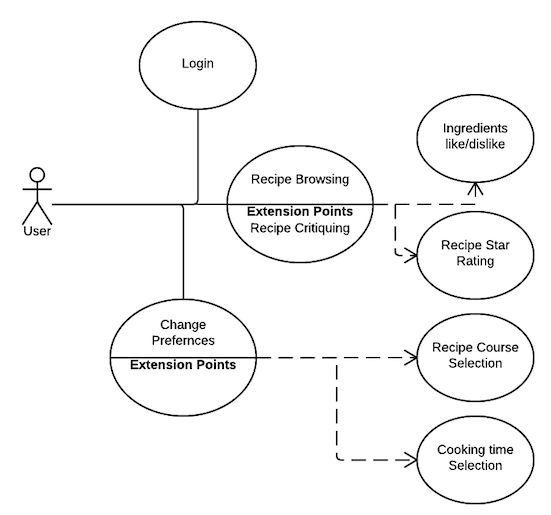
\includegraphics[width=.5\linewidth]{figures/ch4_use_case_foodforme.png}
	\caption{FoodForMe use case diagram}
	\label{fig:ch4_use_case_foodforme}
\end{figure}

\newpage
 
 The first use case, determine user login via Facebook to get his Facebook profile to avoid filling his demographic information by his own. Login flow should provide good user experience and follows the standard practices. Use case start any point of time after app launch and user click on main menu and ends once user can see his name and profile picture at menu screen.  Table \ref{table:import_user-demographic-information} provides the scenario description. \newline
 
 \begin{table}[ht]
 	\centering % used for centering table
 	\begin{tabular}{p{4cm} p{10cm}}  % centered columns (4 columns)
 		\hline\hline %inserts double horizontal lines
 		Use case name & Determine stereotype \\ % inserts table
 		%heading
 		\hline % inserts single horizontal line
 		
		Participating actor & Initiated by User \\ % inserting body of the table
 		Flow of events & (1). User starts app.
 		(2). Click on menu button.
	 	(3). Tap on login via Facebook button to import his Facebook profile. \\
 		Entry condition & User starts app\\
 		Exit condition & User can see his Facebook profile image and name on application slide menu.\\
 		Quality requirements & (1) Import user profile via Facebook SDK. (2) Profile should be import in one click excluding of Facebook login process. (3) It should take more than 30 seconds.\\ [1ex] % [1ex] adds vertical space
 		\hline %inserts single line
 	\end{tabular}
 	\caption{Use case 1:Import user demographic information}
 	\label{table:import_user-demographic-information}
 \end{table}
 
 The second use case, application allow user to logout from application by providing standard mechanism provided by Facebook. After login he is not able to see his personal information in app. Table \ref{table:user_logout} determines the event flow.
  
  \begin{table}[ht]
  	\centering % used for centering table
  	\begin{tabular}{p{4cm} p{10cm}}  % centered columns (4 columns)
  		\hline\hline %inserts double horizontal lines
  		Use case name & Determine stereotype \\ % inserts table
  		%heading
  		\hline % inserts single horizontal line
  		
  		Participating actor & Initiated by User \\ % inserting body of the table
  		Flow of events & 1. User starts app.\newline
  		2. Click on menu button.\newline
  		3. Tap on logout via Facebook button to logout his Facebook profile.\newline
  		4. App shows logout confirmation which includes logout and cancle \\
  		Entry condition & User starts app\\
  		Exit condition & User can logout form applicaiton and unable to his profile picture and name on app menu.\\
  		Quality requirements & 1. User able to logout from system in two clicks.\newline
  		2. It should take more than 30 seconds.\\ [1ex] % [1ex] adds vertical space
  		\hline %inserts single line
  	\end{tabular}
  	\caption{Use case 2: Logout use}
  	\label{table:user_logout}
  \end{table}
 
 Table\ref{table:recipe_browsing} describe use case regarding recipe browsing. According to this user can browse the recipes list that is recommended to him by scrolling up and down. Where recipe list have star rating, recipe name, recipe’s category, review count of recipe.
 
   \begin{table}[ht]
   	\centering % used for centering table
   	\begin{tabular}{p{4cm} p{10cm}}  % centered columns (4 columns)
   		\hline\hline %inserts double horizontal lines
   		Use case name & Determine stereotype \\ % inserts table
   		%heading
   		\hline % inserts single horizontal line
   		
   		Participating actor & Initiated by User \\ % inserting body of the table
   		Flow of events & 1. User can tap on popular/ recommend recipes view.\newline 
   		2. User can see the list of recipes.\newline
   		3. User can perform scrolling to view more recipes.\\
   		Entry condition & User starts app\\
   		Exit condition & User can found his favorite recipe to cook.\\
   		Quality requirements & 1. Scrolling of recipes should be sleek.
   		2. Each item should have name, star rating, avatar or recipe, review count and primary catagory.\\ [1ex] % [1ex] adds vertical space
   		\hline %inserts single line
   	\end{tabular}
   	\caption{Use case 3: Recipe browsing}
   	\label{table:recipe_browsing}
   \end{table}
   
Use case 4 is regarding the showing the detail of selected recipe. This use case is depended use case 3.  On detail screen user can view large image of recipe including all the parameters that is use case 3. Moreover it should display the ingredients along with their quantity. Finally it displays preparation method means how to cook that recipe. Senerios is describe in Table\ref{table:recipe_detail}
   \begin{table}[ht]
   	\centering % used for centering table
   	\begin{tabular}{p{4cm} p{10cm}}  % centered columns (4 columns)
   		\hline\hline %inserts double horizontal lines
   		Use case name & Determine stereotype \\ % inserts table
   		%heading
   		\hline % inserts single horizontal line
   		
   		Participating actor & Initiated by User \\ % inserting body of the table
   		Flow of events & 1. User selects recipe from list (Use case 3)\newline 
   		2. User can see ingredients of selected recipe along with quantity.\newline
   		3. User can cooking method\\
   		Entry condition & User select a recipe from recommended item\\
   		Exit condition & User can found his favorite recipe to cook.\\
   		Quality requirements & 1. Scrolling of recipe should be sleek. 2. Each item should have cooking method and set of ingredients along with quantity\\ [1ex] % [1ex] adds vertical space
   		\hline %inserts single line
   	\end{tabular}
   	\caption{Use case 4: Recipe Detail}
   	\label{table:recipe_detail}
   \end{table}
   
   Use case 5 of our system is critiquing a recipe. System allows user to critique on user’s recommend recipe so that system will aware about user taste and his health need. In our system critiquing of recipe and its ingredient is down by separately so that we can evaluate user taste more specifically. It might be possible that user doesn’t like the recipe but his likes the ingredient and those ingredients are the essential one for his dietary need. Therefore, recipe critiquing is done via star rating where ingredient can be critique by like/dislike. Table \ref{table:recipe_ingredient_critique} discuss the event flow of this use case.
   
   
    \begin{table}[ht]
    	\centering % used for centering table
    	\begin{tabular}{p{4cm} p{10cm}}  % centered columns (4 columns)
    		\hline\hline %inserts double horizontal lines
    		Use case name & Determine stereotype \\ % inserts table
    		%heading
    		\hline % inserts single horizontal line
    		
    		Participating actor & Initiated by User \\ % inserting body of the table
    		Flow of events & 1. User is viewing recipe detail 
			He wants to give his feed back about recommend recipe. 
			2. He taps on Critique button at top right corner of recipe detail screen. 
			3. On critique screen he may like/dislike ingredients. 
			4. He may rate recipe by selecting stars.\\
    		Entry condition & use case 1, 3, 4\\
    		Exit condition & User can found his favorite recipe to cook.\\
    		Quality requirements & 1. Like/dislike have differnt color 2. Rating of recipe is done via stars selection\\ [1ex] % [1ex] adds vertical space
    		\hline %inserts single line
    	\end{tabular}
    	\caption{Use case 5: Recipe Critique}
    	\label{table:recipe_ingredient_critique}
    \end{table}
    
    
\section{User interface}    


\subsection{Main Menu}
\begin{figure}[h]
	\begin{subfigure}{.49\textwidth}
		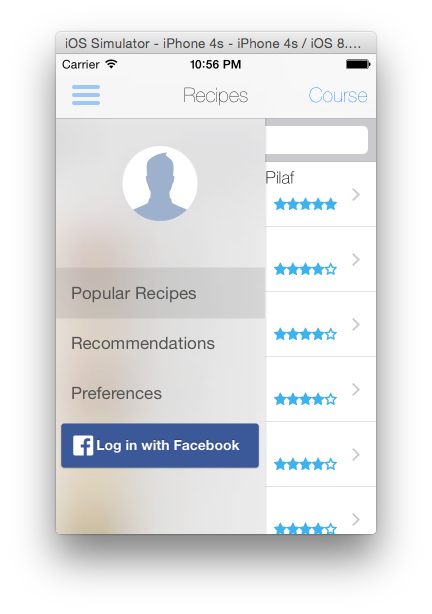
\includegraphics[width=.9\linewidth]{figures/ch4_app_screen_shots/main_menu/main_menu_1.png}
		\caption{Logout user}
		%\label{fig:ch2_lamche2014active_1}
	\end{subfigure}
	\begin{subfigure}{.49\textwidth}
		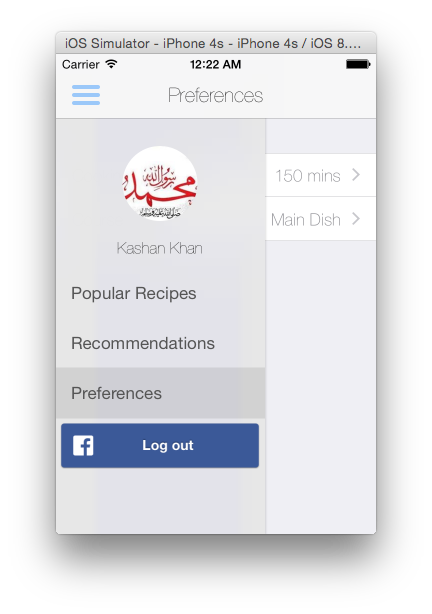
\includegraphics[width=.9\linewidth]{figures/ch4_app_screen_shots/main_menu/main_menu_2.png}
		\caption{Login user}
		%\label{fig:ch2_lamche2014active_2}
	\end{subfigure}
	\caption{FoodForMe Main Menu}
	\label{fig:foodforme_main_menu_sreen}
\end{figure}
	  
\subsection{Popular/Recommended Recipes}
 \begin{figure}[h]
 	\centering
	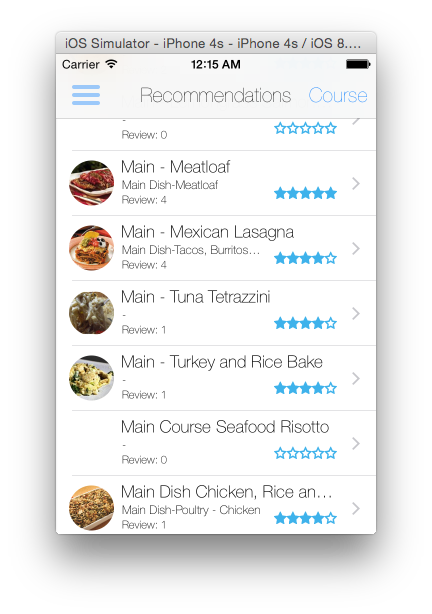
\includegraphics[width=.5\linewidth]{figures/ch4_app_screen_shots/recipes/recipes.png}
    \caption{FoodForMe use case diagram}
	\label{fig:foodforme_recipe_screen}
	\end{figure}
	  
\subsection{Recipe Detail} 
	  \begin{figure}[h]
	  	\begin{subfigure}{.32\textwidth}
	  		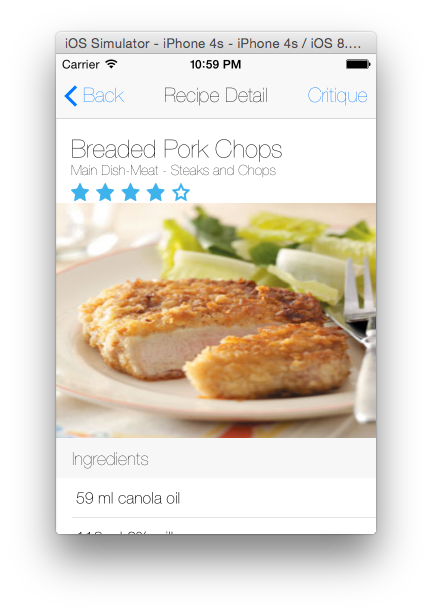
\includegraphics[width=.9\linewidth]{figures/ch4_app_screen_shots/recipe_detail/recipe_detail_1.png}
	  		\caption{Logout user}
	  		%\label{fig:ch2_lamche2014active_1}
	  	\end{subfigure}
	  	\begin{subfigure}{.32\textwidth}
	  		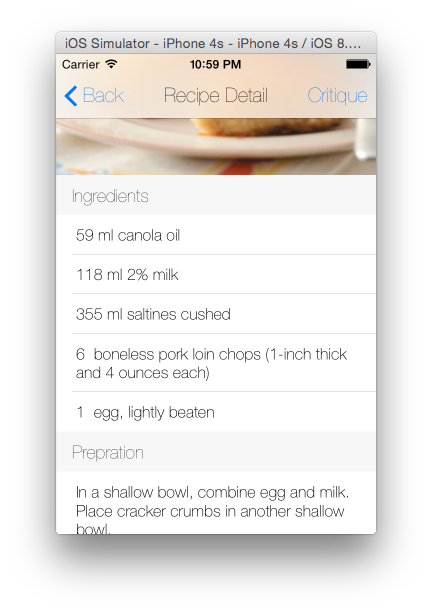
\includegraphics[width=.9\linewidth]{figures/ch4_app_screen_shots/recipe_detail/recipe_detail_2.png}
	  		\caption{Login user}
	  		%\label{fig:ch2_lamche2014active_2}
	  	\end{subfigure}
	  	\begin{subfigure}{.32\textwidth}
	  		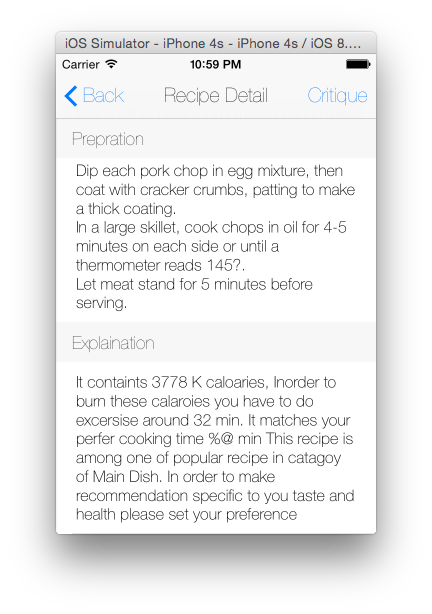
\includegraphics[width=.9\linewidth]{figures/ch4_app_screen_shots/recipe_detail/recipe_detail_3.png}
	  		\caption{Login user}
	  		  		%\label{fig:ch2_lamche2014active_2}
		  	\end{subfigure}
	  	\caption{FoodForMe Recipe Detail}
	  	\label{fig:foodforme_main_menu_sreen}
	  \end{figure}
%%%%%%%% recipe_detail
%
%figures/ch4_app_screen_shots/recipe_detail/recipe_detail_2.png
%figures/ch4_app_screen_shots/recipe_detail/recipe_detail_3.png

%figures/ch4_app_screen_shots/recipe_detail/recommended_recipe_explaination/recommended_recipe_explaination_1.png
%figures/ch4_app_screen_shots/recipe_detail/recommended_recipe_explaination/recommended_recipe_explaination_2.png
\subsubsection{explanation}
\begin{figure}[h]
	\begin{subfigure}{.49\textwidth}
		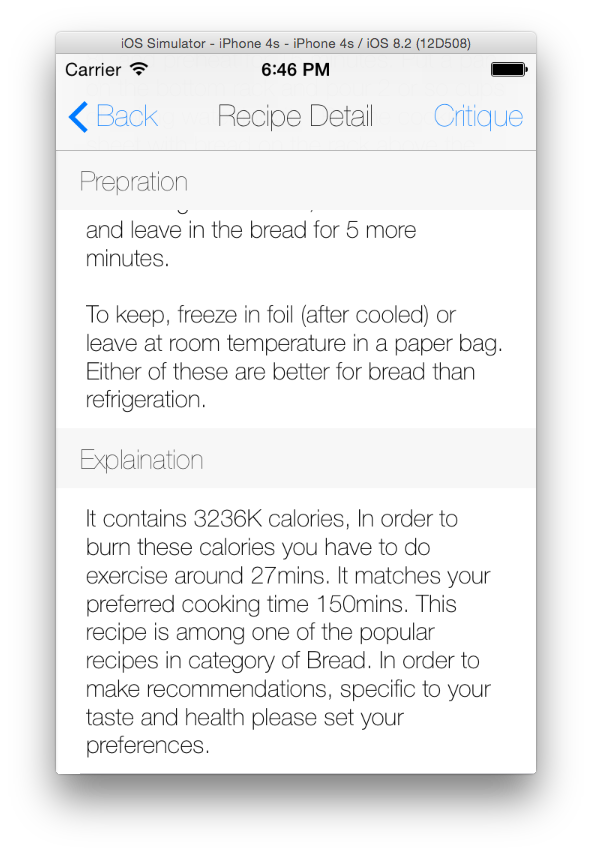
\includegraphics[width=.9\linewidth]{figures/ch4_app_screen_shots/recipe_detail/recommended_recipe_explaination/recommended_recipe_explaination_1.png}
		\caption{Logout user}
		%\label{fig:ch2_lamche2014active_1}
	\end{subfigure}
	\begin{subfigure}{.49\textwidth}
		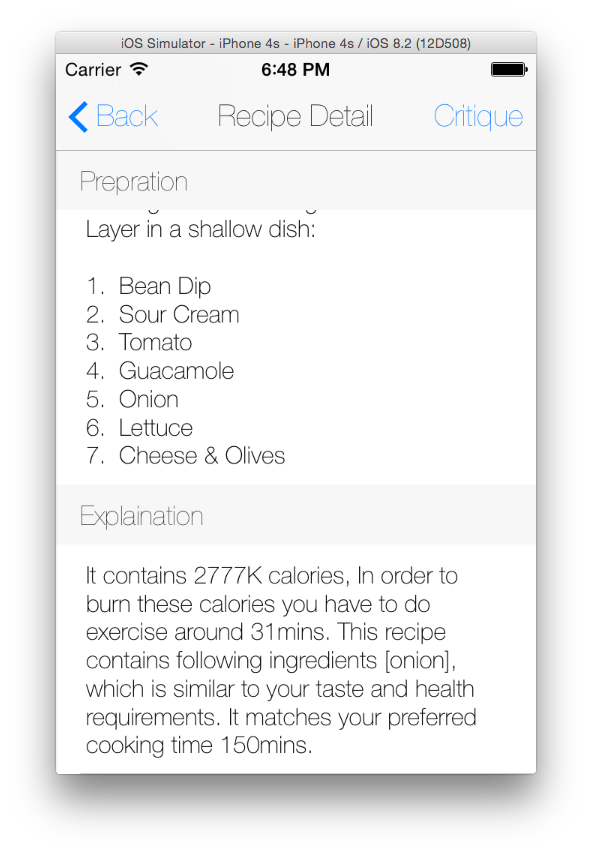
\includegraphics[width=.9\linewidth]{figures/ch4_app_screen_shots/recipe_detail/recommended_recipe_explaination/recommended_recipe_explaination_2.png}
		\caption{Login user}
		%\label{fig:ch2_lamche2014active_2}
	\end{subfigure}
	\caption{FoodForMe Main Menu}
	\label{fig:foodforme_main_menu_sreen}
\end{figure}


\subsection{Recipe critiquing} 
%%%%% critique
%
%figures/ch4_app_screen_shots/critique/critique_2.png
%figures/ch4_app_screen_shots/critique/critique_3.png
%figures/ch4_app_screen_shots/critique/critique_4.png


	  \begin{figure}[h]
	  	\begin{subfigure}{.32\textwidth}
	  		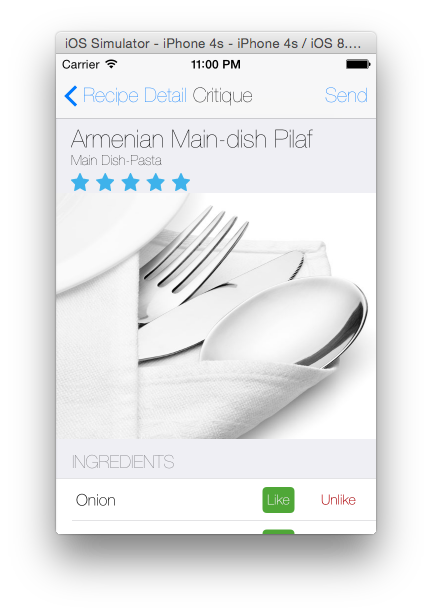
\includegraphics[width=.9\linewidth]{figures/ch4_app_screen_shots/critique/critique_1.png}
	  		\caption{Logout user}
	  		%\label{fig:ch2_lamche2014active_1}
	  	\end{subfigure}
	  	\begin{subfigure}{.32\textwidth}
	  		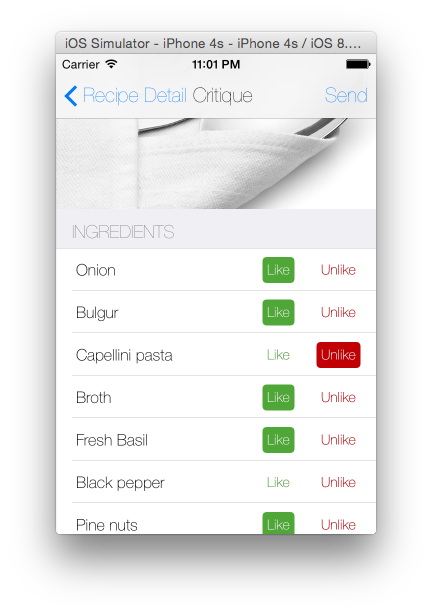
\includegraphics[width=.9\linewidth]{figures/ch4_app_screen_shots/critique/critique_2.png}
	  		\caption{Login user}
	  		%\label{fig:ch2_lamche2014active_2}
	  	\end{subfigure}
	  	\begin{subfigure}{.32\textwidth}
	  		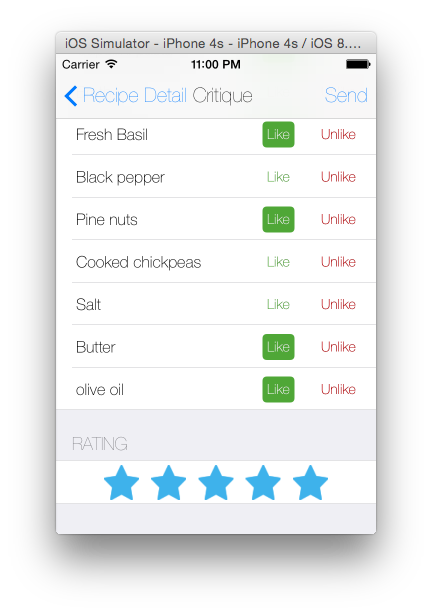
\includegraphics[width=.9\linewidth]{figures/ch4_app_screen_shots/critique/critique_4.png}
	  		\caption{Login user}
	  		  		%\label{fig:ch2_lamche2014active_2}
	  		\end{subfigure}
	  	\caption{FoodForMe Recipe Detail}
	  	\label{fig:foodforme_main_menu_sreen}
	  \end{figure}

%%%%%%%% preferences
%figures/ch4_app_screen_shots/preferences/peferences.png
%figures/ch4_app_screen_shots/preferences/peferences_course.png
%figures/ch4_app_screen_shots/preferences/peferences_cooking_time.png
\subsection{Preferences} 
	  \begin{figure}[h]
	  	\begin{subfigure}{.32\textwidth}
	  		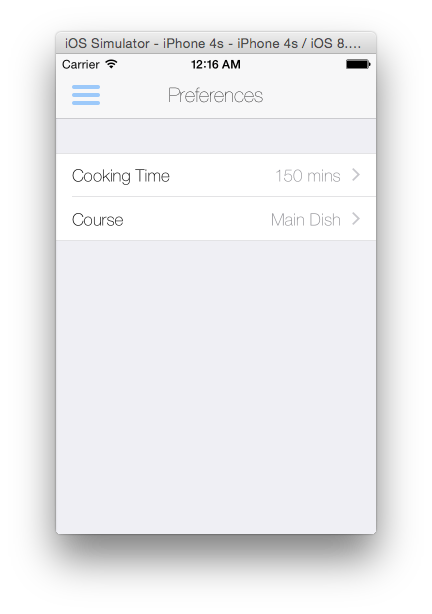
\includegraphics[width=.9\linewidth]{figures/ch4_app_screen_shots/preferences/peferences.png}
	  		\caption{Logout user}
	  		%\label{fig:ch2_lamche2014active_1}
	  	\end{subfigure}
	  	\begin{subfigure}{.32\textwidth}
	  		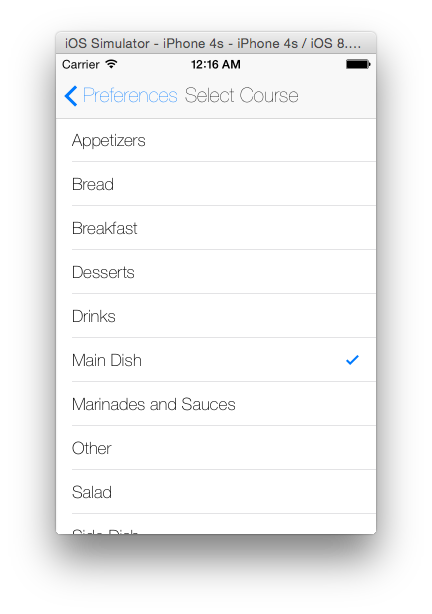
\includegraphics[width=.9\linewidth]{figures/ch4_app_screen_shots/preferences/peferences_course.png}
	  		\caption{Login user}
	  		%\label{fig:ch2_lamche2014active_2}
	  	\end{subfigure}
	  	\begin{subfigure}{.32\textwidth}
	  		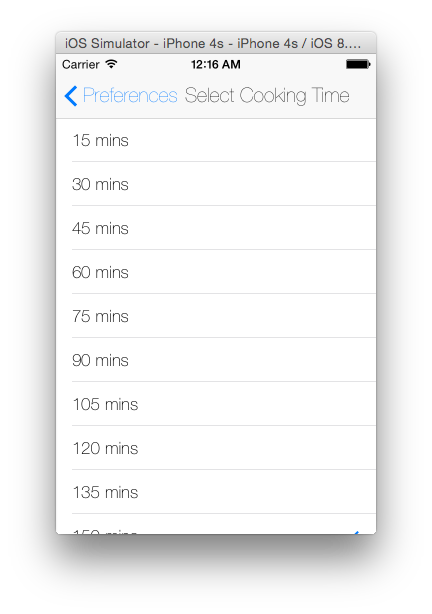
\includegraphics[width=.9\linewidth]{figures/ch4_app_screen_shots/preferences/peferences_cooking_time.png}
	  		\caption{Login user}
	  		%\label{fig:ch2_lamche2014active_2}
	  	\end{subfigure}
	  	\caption{FoodForMe Recipe Detail}
	  	\label{fig:foodforme_main_menu_sreen}
	  \end{figure}
	  
\section*{FoodForMe iOS Data Model}	  
	   \begin{figure}[h]
	   	\centering
	   	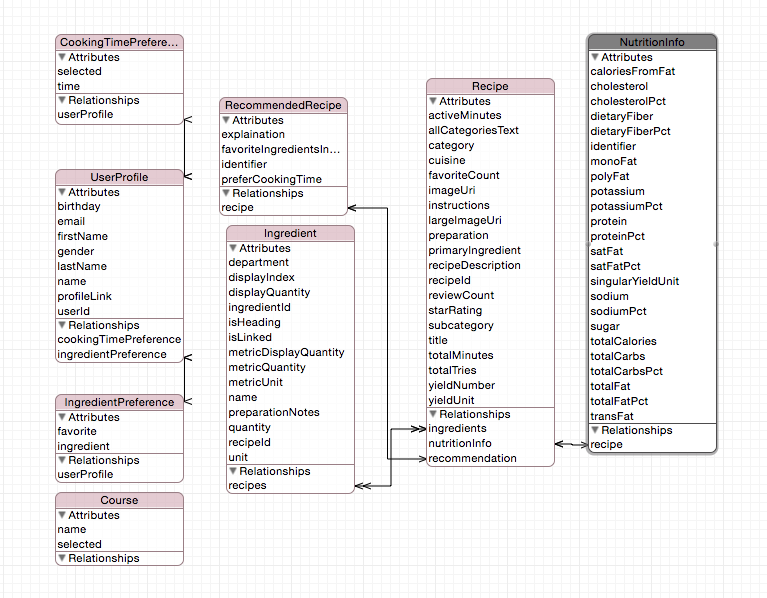
\includegraphics[width=1\linewidth]{figures/ch4_ios_data_model}
	   	\caption{FoodForMe use case diagram}
	   	\label{fig:foodforme_recipe_screen}
	   \end{figure}
	   
	  
	  
\section{System Architecture}

\subsection{Working}

\subsection{Class Drigram}

\subsection{ERD}

\section{System Services}

\subsection{Service 1}
